\documentclass[border=4pt]{standalone}
\usepackage{fontspec}
\usepackage{amsmath}
\usepackage{unicode-math}
\setmainfont{Latin Modern Roman}
\setmathfont{Latin Modern Math}
\usepackage{pgfplots}
\usepackage{pgfplotstable}
\pgfplotsset{compat=1.18}
\usepackage{tkz-euclide}
\usetikzlibrary{arrows.meta,calc,angles,quotes,patterns,3d,backgrounds}
\definecolor{ink}{HTML}{123428}
\definecolor{asy}{HTML}{475569}
\definecolor{mint}{HTML}{86e0bd}
\tikzset{asym/.style={asy, line width=0.9pt, dash pattern=on 5pt off 3.5pt},
         guide/.style={gray!70, line width=0.6pt, densely dotted},
         dot/.style={circle, inner sep=0pt, minimum size=5pt, draw=white, line width=0.5pt},
         odot/.style={circle, inner sep=0pt, minimum size=5.5pt, fill=white, line width=1pt},
         lab/.style={font=\footnotesize, inner sep=1.5pt, text=ink}}
\begin{document}
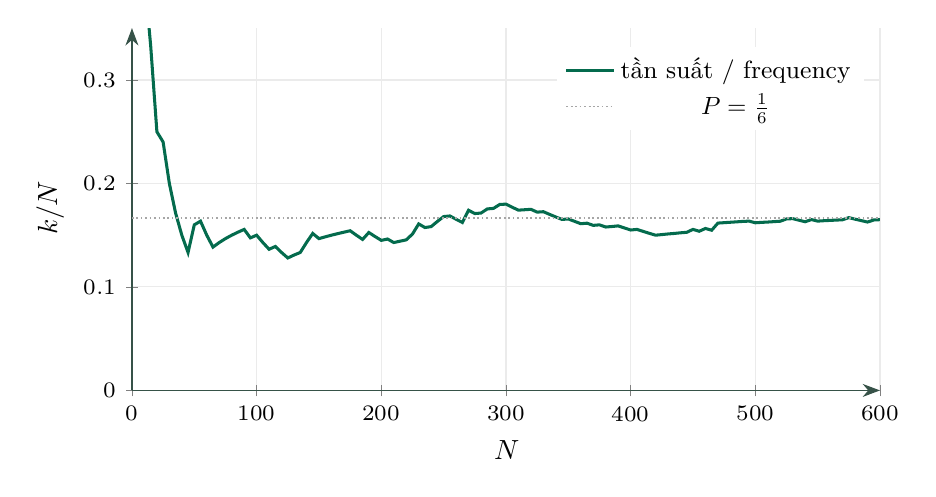
\begin{tikzpicture}\begin{axis}[scale only axis, width=9.5cm, height=4.6cm, xmin=0, xmax=600, ymin=0, ymax=0.35, axis lines=left,
 axis line style={draw=ink!85, -{Stealth[length=2.2mm]}}, xlabel={$N$}, ylabel={$k/N$}, grid=major, major grid style={draw=gray!16}, ticklabel style={font=\footnotesize},
 yticklabel style={/pgf/number format/fixed}, legend style={at={(0.98,0.95)}, anchor=north east, draw=none, fill=white, font=\small}]
\addplot[color={rgb,255:red,4;green,107;blue,77}, line width=1.1pt] coordinates {(5,0.4000) (10,0.4000) (15,0.3333) (20,0.2500) (25,0.2400) (30,0.2000) (35,0.1714) (40,0.1500) (45,0.1333) (50,0.1600) (55,0.1636) (60,0.1500) (65,0.1385) (70,0.1429) (75,0.1467) (80,0.1500) (85,0.1529) (90,0.1556) (95,0.1474) (100,0.1500) (105,0.1429) (110,0.1364) (115,0.1391) (120,0.1333) (125,0.1280) (130,0.1308) (135,0.1333) (140,0.1429) (145,0.1517) (150,0.1467) (155,0.1484) (160,0.1500) (165,0.1515) (170,0.1529) (175,0.1543) (180,0.1500) (185,0.1459) (190,0.1526) (195,0.1487) (200,0.1450) (205,0.1463) (210,0.1429) (215,0.1442) (220,0.1455) (225,0.1511) (230,0.1609) (235,0.1574) (240,0.1583) (245,0.1633) (250,0.1680) (255,0.1686) (260,0.1654) (265,0.1623) (270,0.1741) (275,0.1709) (280,0.1714) (285,0.1754) (290,0.1759) (295,0.1797) (300,0.1800) (305,0.1770) (310,0.1742) (315,0.1746) (320,0.1750) (325,0.1723) (330,0.1727) (335,0.1701) (340,0.1676) (345,0.1652) (350,0.1657) (355,0.1634) (360,0.1611) (365,0.1616) (370,0.1595) (375,0.1600) (380,0.1579) (385,0.1584) (390,0.1590) (395,0.1570) (400,0.1550) (405,0.1556) (410,0.1537) (415,0.1518) (420,0.1500) (425,0.1506) (430,0.1512) (435,0.1517) (440,0.1523) (445,0.1528) (450,0.1556) (455,0.1538) (460,0.1565) (465,0.1548) (470,0.1617) (475,0.1621) (480,0.1625) (485,0.1629) (490,0.1633) (495,0.1636) (500,0.1620) (505,0.1624) (510,0.1627) (515,0.1631) (520,0.1635) (525,0.1657) (530,0.1660) (535,0.1645) (540,0.1630) (545,0.1651) (550,0.1636) (555,0.1640) (560,0.1643) (565,0.1646) (570,0.1649) (575,0.1670) (580,0.1655) (585,0.1641) (590,0.1627) (595,0.1647) (600,0.1650)};
\addlegendentry{tần suất / frequency}
\addplot[guide, domain=0:600, samples=2] {1/6}; \addlegendentry{$P=\frac16$}
\end{axis}\end{tikzpicture}
\end{document}
